\chapter{Dataset}

In this chapter, we will discuss the dataset used for the project, the data augmentation techniques used to increase the size of the dataset and the data preprocessing techniques used to prepare the dataset for the model.


\section*{Dataset}
The dataset used for this project comes from Kaggle: \textit{Pothole Segmentation YOLOv8}. 

It is a dataset of 780 images of potholes, 720 of which are used for training and 60 for testing. 
The images are in the format of 640x640 pixels and are annotated in YOLOv8 format. 

In order to increase the size of the dataset, for each image, there are 3 versions with different augmentations between:
\begin{itemize}
    \item 50\% probability of horizontal flip
    \item Randomly crop between 0 and 20 percent of the image
    \item Random rotation of between -15 and +15 degrees
    \item Random shear of between -5° to +5° horizontally and -5° to +5° vertically
    \item Random brigthness adjustment of between -25 and +25 percent
    \item Random exposure adjustment of between -25 and +25 percent
\end{itemize}



\subsection*{Labelling}
The dataset is annotated in YOLOv8 format.
For each image, there is a corresponding text file with the same name where each line correspond to a pothole in the image. Each one of those lines contains the following information:
\begin{itemize}
    \item The class of the object (in this case, the class is always 0, as there is only one class: pothole);
    \item A list of couple of coordinates $[x, y]$ that represent a point of the shape of the pothole. The union of all these points represents the mask. The coordinates are normalized, so they are in the range $[0, 1]$.
\end{itemize}
An example of the content of a text file with the corresponding points projections is shown in Figure \ref{fig:annotation_example}.


\begin{figure}[!htb]
    \begin{minipage}{0.48\textwidth}
      \centering
      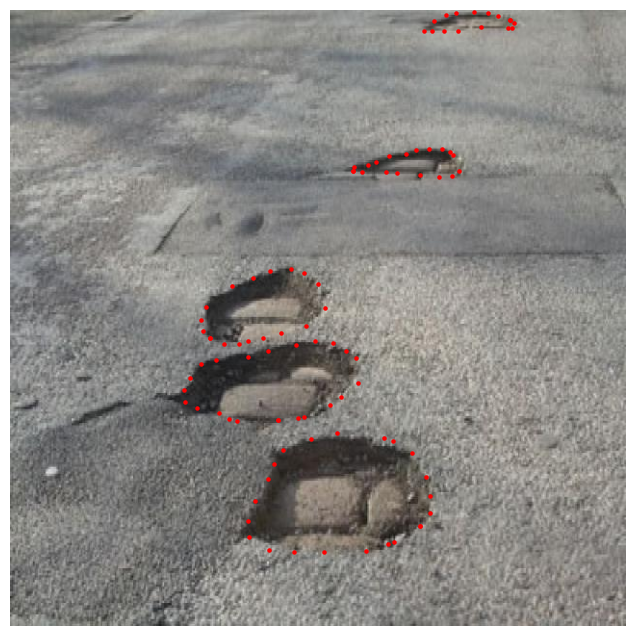
\includegraphics[width=.9\linewidth]{Images/pothole_yolov8_example.png}
    \end{minipage}\hfill
    \begin{minipage}{0.5\textwidth}
      \centering
      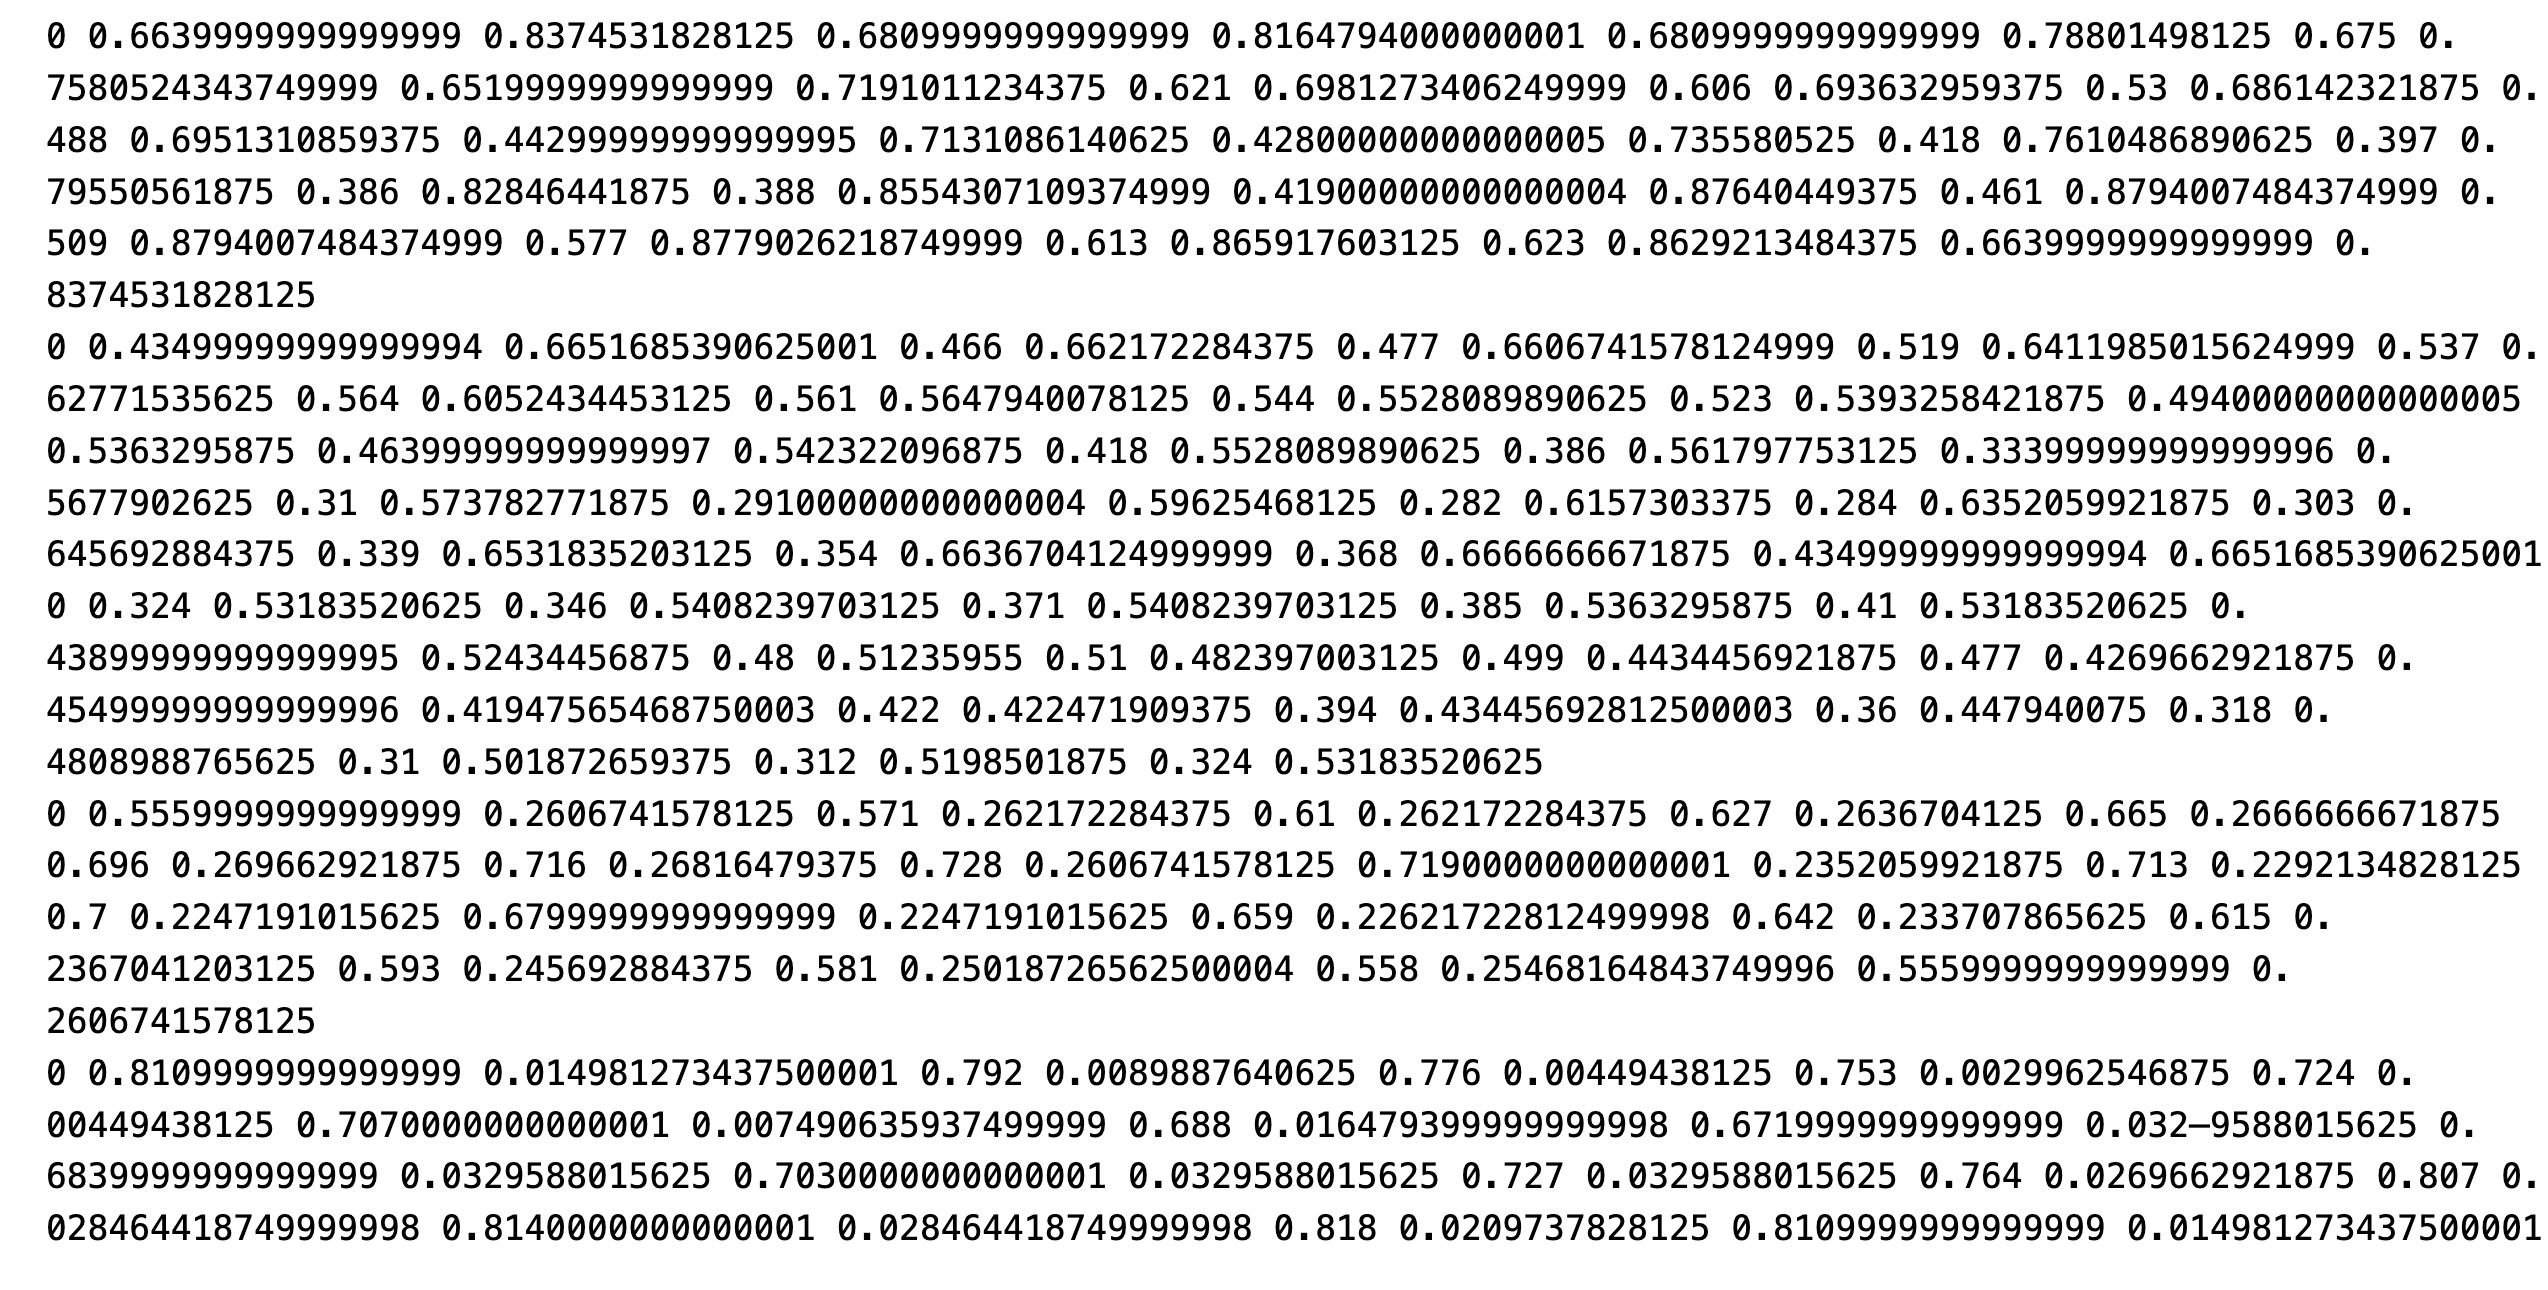
\includegraphics[width=1.1\linewidth]{Images/annotation_example.jpg}
    \end{minipage}
    \caption{On the right, an example of the content of a label file. On the left, the corresponding image with the projection of the points.}
    \label{fig:annotation_example}
 \end{figure}

\section{Data Conversion}
Since the model used in this project is Mask R-CNN, the dataset needs to be converted to the COCO format. \\

The COCO format is a JSON file that contains all the information about the dataset, including the images, the annotations, the categories, and the information about the licenses.
The conversion is done using the function \textit{generateJSON} that takes as input the path of the dataset and the path where the COCO file will be saved. \\\\
\begin{figure}[ht]
    \centering
    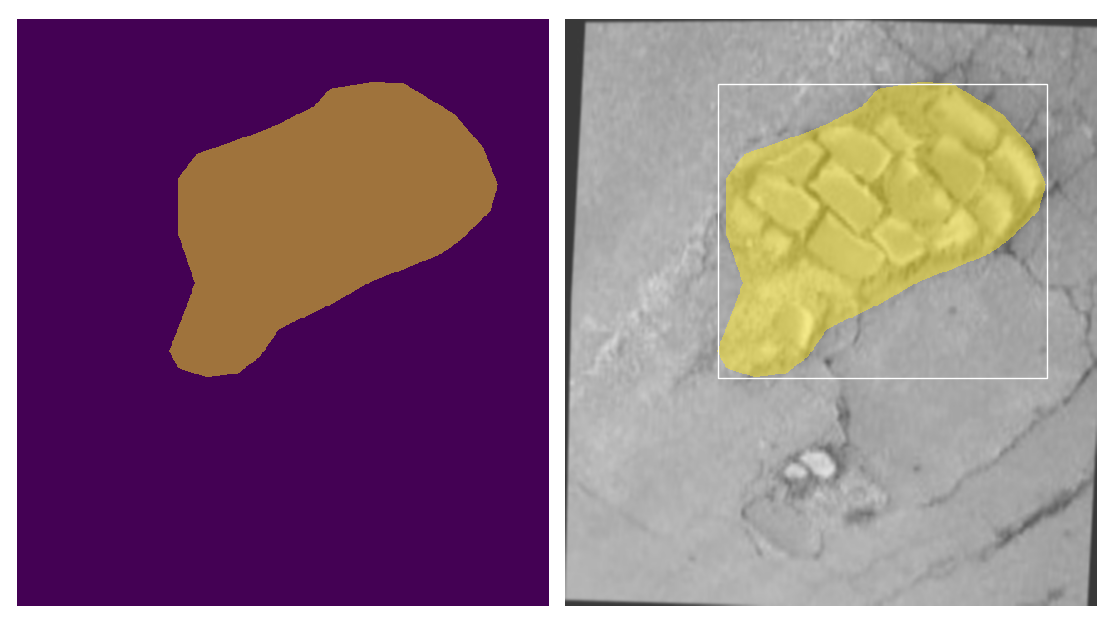
\includegraphics[width=0.7\textwidth]{Images/sample.png}
    \caption{Example of the images after the augmentation. On the left the resulting mask, on the right the original image with labels.}
    \label{fig:augmentation_example}
\end{figure}

The json file is structured as follows:
\begin{itemize}
    \item \textit{images}: contains information about all the images such as dimensions and file name;
    \item \textit{annotations}: contains various metadata informations and the main information about the pothole:
        \begin{itemize}
            \item \textit{segmentation}: contains the mask of the pothole in the format of a list of points $[x, y]$;
            \item \textit{bbox}: contains the bounding box of the pothole in the format $[x, y, w, h]$;
        \end{itemize}
\end{itemize}

\section{Data Augmentation}
The dataset used for this project is quite small, even after the augmentation done by the authors. To tackle this problem, we used data augmentation techniques to increase the size of the dataset.
In particular, we just used the following techniques:
\begin{itemize}
    \item Horizontal flip with a probability of 50\%;
    \item Vertical flip with a probability of 50\%;
\end{itemize}

We also give a custom implementation of the \textit{Gaussian Blur} filter and the \textit{Gaussian Noise} filter. The first one is used to simulate the blur that can be present in the images due to the motion of the camera or the presence of rain: for this reason, the filter is applied also with the purpose of increasing the model generalization and performance. 
The latter is actually not used in the final implementation of the model, but it is still present in the code. The reason behind this is because the Gaussian Noise is a heavy filter that can change drastically the image: experiments showed that the model could not learn well enough and performance suffered.

We show an example of the images after the augmentation in Figure \ref{fig:augmentation_example}.
